\subsection{Visualization} % (fold)
\label{sub:visualization}

The greatest challenge of this work was the creation of the visualization part for its requirements. We will now overview this part of Eagle Eye, its architecture, visualization techniques, sorting and filtering capabilities.

\subsubsection{Overview}
We wanted to make the visualization simple and easy to use, while keeping it flexible and capable enough to allow for an enjoyable and relevant experience.

After the backend has finished processing, the visualization can be opened and all will appear in ``the canvas''. After loading the metadata, the user is also presented with a set of options on the toolbar (\fig{viz5679images}).


\begin{figure}[ht]
	\centering
		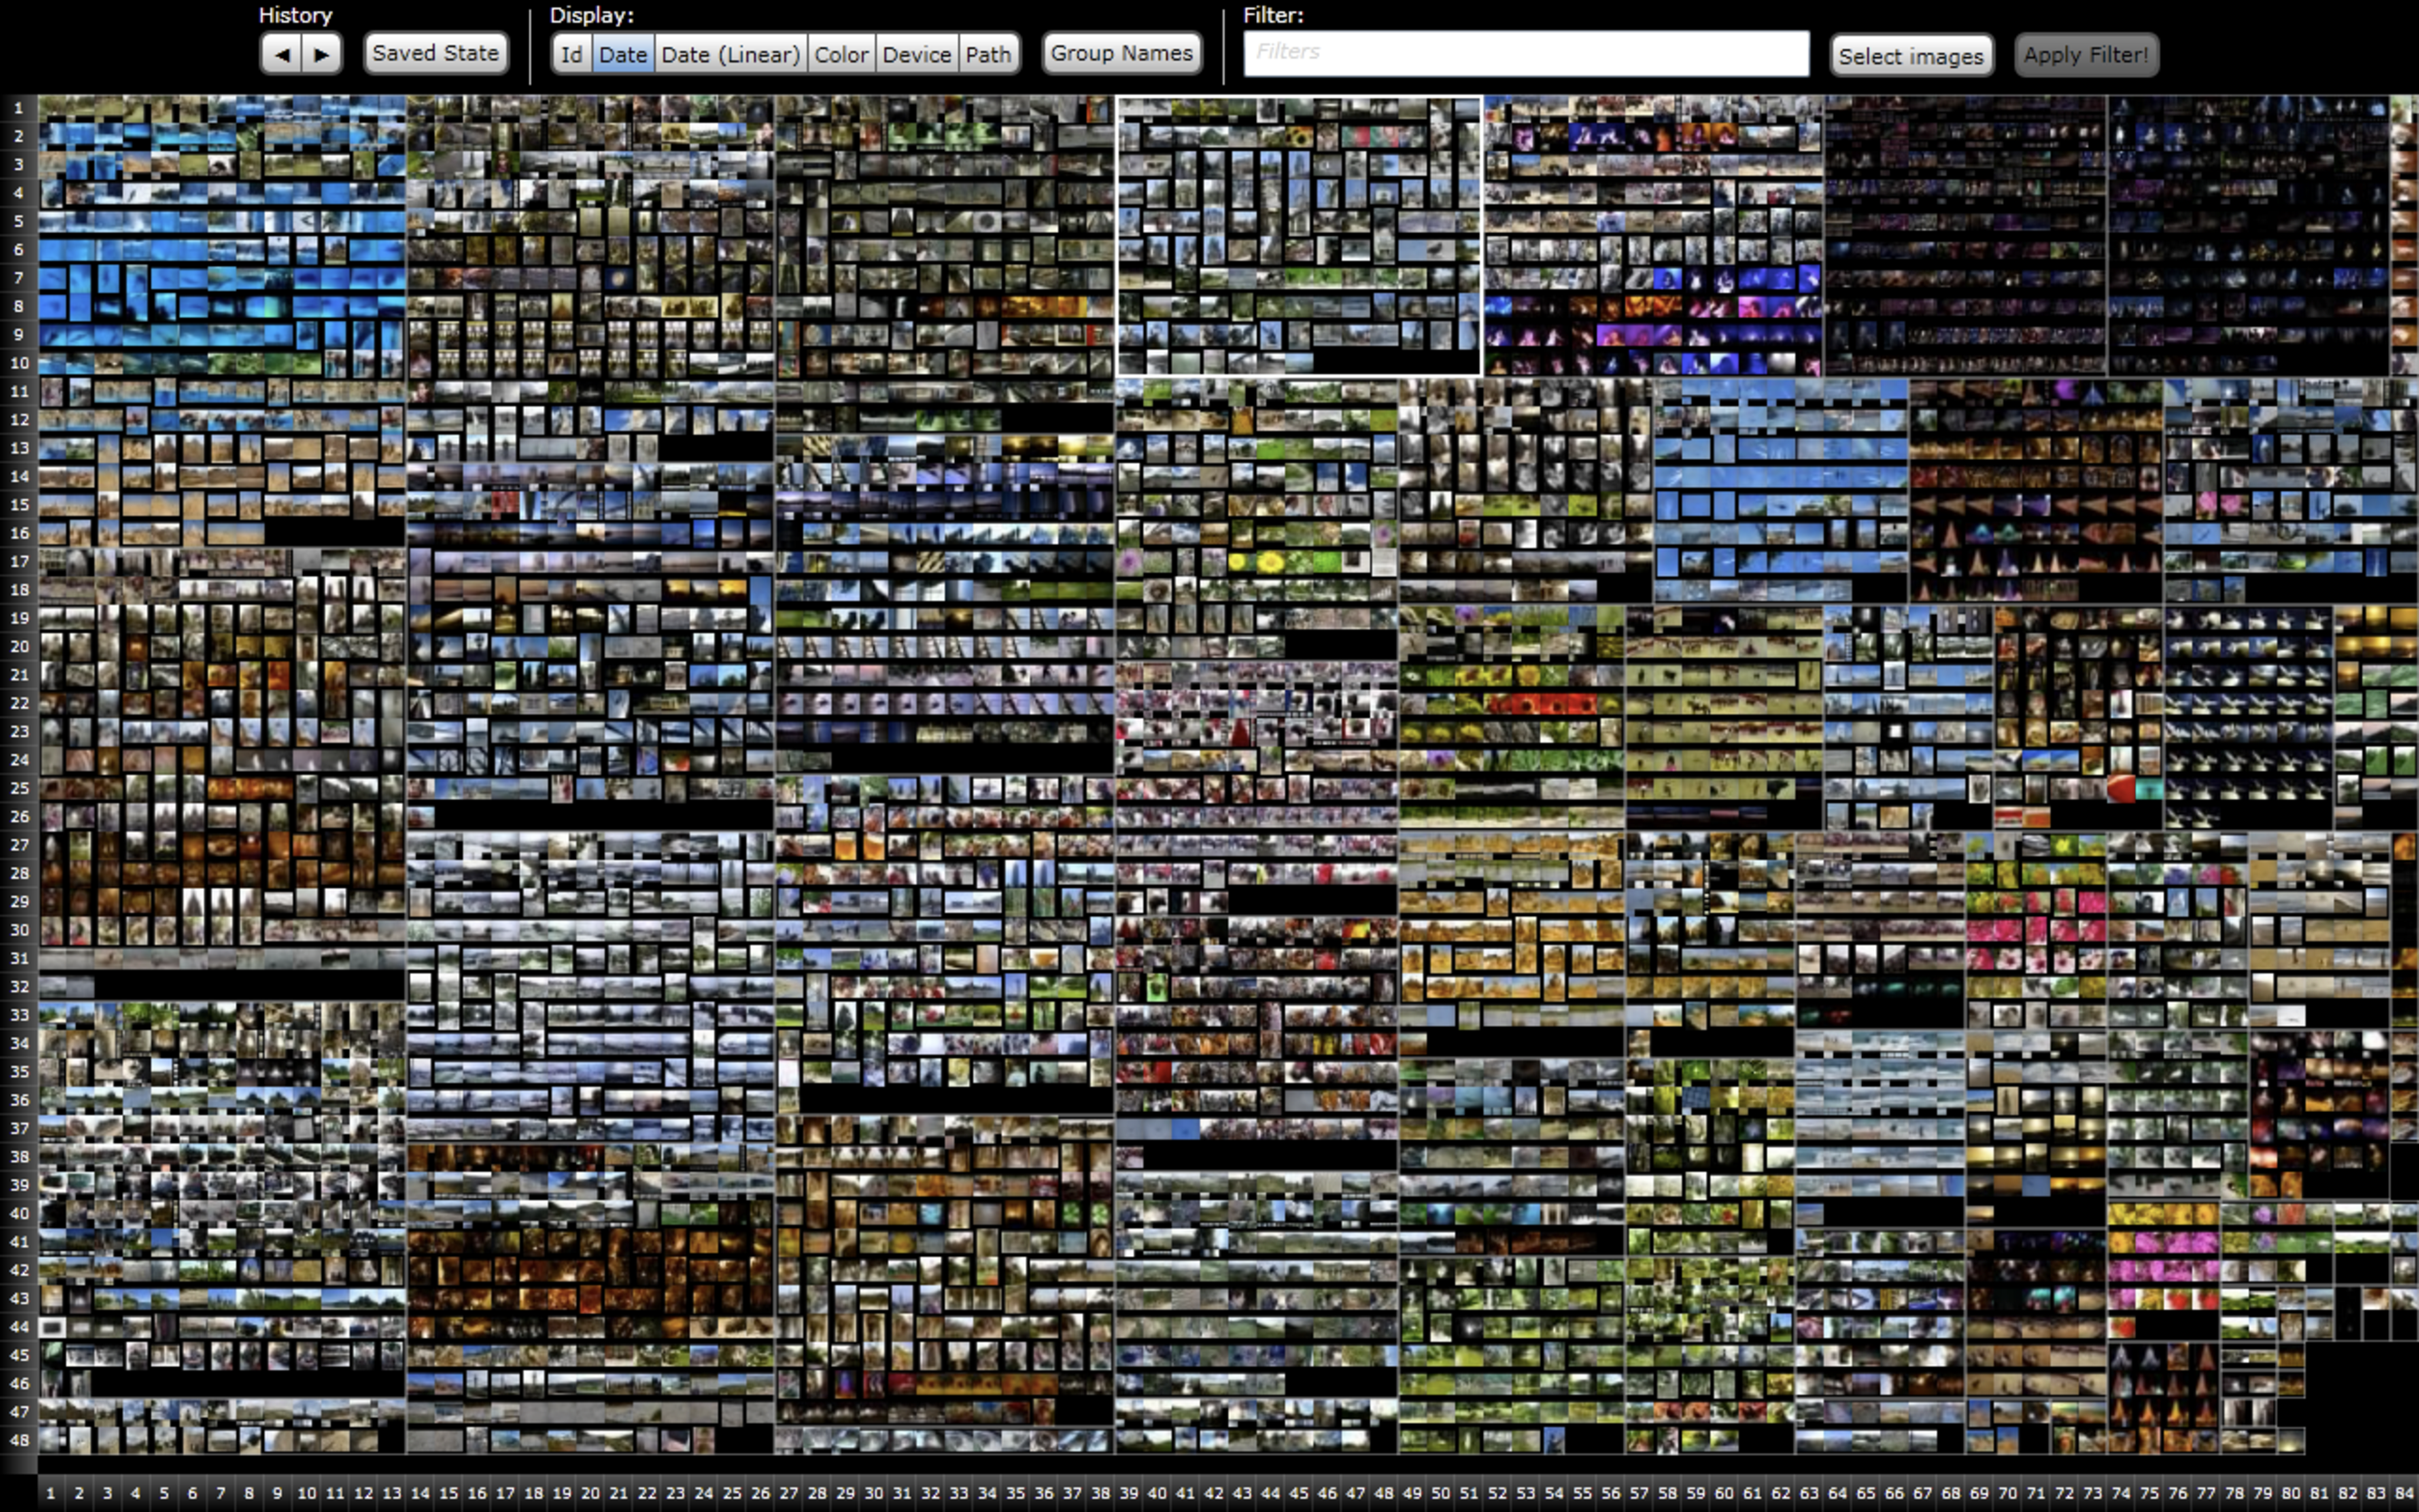
\includegraphics[width=\columnwidth]{../Figures/viz5679images1280.pdf}
	\caption{Example of the visualization of 5679 images, organized by capture date, in Eagle Eye.}
	\label{fig:viz5679images}
\end{figure}



\textbf{The Canvas} is the most relevant part of the visualization as it displays the user's images.

Eagle Eye displays images very small, but because the interest is in users viewing their own collections, they user recalls what is that image without having to understand a totally new image. The grouping of events (e.g. by date or path) also helps the user to extrapolate the contents of the whole group from looking at a few of them instead of trying to understand each image individually. This allows much faster recognition of groups with small images.

Eagle Eye allows manipulation of the canvas by panning and zooming up to fullscreen images.


%%%%%%%%%%%%%%%%%%%%%%%%%%%%%%%%
\textbf{The toolbar}
The user can use the functions on the toolbar to filter and sort differently.



\subsubsection{Disposition of Images on Canvas}
\label{sub:dispositions}

We have come up with a some options for photo grouping, sorting and filtering.

\textbf{Sorting images into groups} Eagle Eye currently groups together images captured at the same day, with the same median color, from the same path or with the same number of faces, depending on user choice.

\textbf{Different dispositions} We implemented a Treemap for displaying most of different groupping options. This treemap is aware of the constraints of dealing with images. We also implemented a ``linear'' display for displaying images sequentially.

\textbf{Filtering} % (fold)
Eagle Eye also provides the user with the ability to filter images in two ways, using the filter bar for textual filtering or selecting pictures on the canvas.



\subsubsection{Architecture of the Visualization}

We will now take a look into the architecture of the visualization part of Eagle Eye.


\textbf{Metadata indexing} The visualization uses metadata embedded by the backend, which is obtained, parsed and indexed for later use.

\textbf{Canvas} is a wrapper for the DeepZoom display. It stores settings and images positions and computes new ones. It also uses memoization to avoid repeated calculations.

\textbf{Reducing Clutter} Eagle Eye groups images that were taken within an interval of 4 seconds. A whole group is reduced to the space of one image, keeping the first one at its normal size, but not centered on the grid. The resulting space left is used for the other images. The user can always zoom in to see them.